\chapter{C 语言的基本功}
\label{chap:c-basics}

上一章，我们把 Hello, world 当成模板，在中间写 \texttt{printf}，让计算机打印出想打印的东西。这一章，我们要让程序真正“动”起来：会记住数，会算数，会读入你敲的键盘，会做决定，还会不知疲倦地重复做同一件事。

学完这些，程序就能做很多事了。本章最后，我们会只用这些最基本的东西，写一个可以玩的文字冒险游戏。

本章的所有示例都在 \texttt{code/ch02/} 目录中。在 WSL 或 Linux 终端中进入这个目录，运行 \texttt{make} 编译全部程序，运行 \texttt{make test} 可以自动检查每个程序的输出。书中显示的运行结果，都是这些程序真正运行的结果。

\section{变量：贴了标签的盒子}
\label{sec:variable}

\codefile{code/ch02/var.c}{变量和加法}{lst:var}

运行结果：
\inputminted[linenos=false]{text}{code/ch02/out/var.txt}

\texttt{int a = 3;} 的意思是：准备一个能装整数的盒子，贴上标签 \texttt{a}，往里面放进 3。这个盒子就是\emph{变量}，标签就是变量的名字，盒子里装的东西是变量的\emph{值}（图~\ref{fig:boxes}）。\texttt{int} 是 integer（整数）的缩写，说明这个盒子只能装整数。

\begin{figure}[htbp]
  \centering
  \begin{tikzpicture}[line width=0.8pt]
    \foreach \x/\n/\v in {0/a/3, 2.9/b/4, 5.8/c/7} {
      \filldraw[fill=brown!30]  (\x,0) rectangle +(1.6,1.2);
      \filldraw[fill=brown!15]  (\x,1.2) -- +(0.4,0.3) -- +(2.0,0.3) -- +(1.6,0) -- cycle;
      \filldraw[fill=brown!45]  (\x+1.6,0) -- +(0.4,0.3) -- +(0.4,1.5) -- +(0,1.2) -- cycle;
      \node[font=\huge\bfseries] at (\x+0.8,0.6) {\v};
      \node[draw, fill=yellow!40, rotate=8, font=\ttfamily\large,
            inner sep=3pt] at (\x+0.8,-0.4) {\n};
    }
    \node[font=\huge] at (2.45,0.7) {+};
    \node[font=\huge] at (5.35,0.7) {=};
    \node[font=\small, align=left, anchor=west] at (8.0,1.0)
      {\texttt{c = a + b;}\\[2pt]把 a、b 盒子里的数相加，\\放进 c 盒子};
  \end{tikzpicture}
  \caption{变量就像一个个贴了标签的盒子}
  \label{fig:boxes}
\end{figure}

\texttt{int c;} 只准备了盒子，没有往里面放东西。这时 \texttt{c} 里装的是什么？谁也不知道，可能是任何一个数。所以在用一个变量之前，一定要先给它一个值。

\texttt{c = a + b;} 先取出 \texttt{a} 和 \texttt{b} 的值，算出 $3 + 4 = 7$，再把 7 放进 \texttt{c}。注意，C 语言里的 \texttt{=} 不是数学里的“等于”，而是“放进去”的意思，叫做\emph{赋值}。所以 \texttt{a = 10;} 把 \texttt{a} 里原来的 3 倒掉，换成 10。在数学里，下面这个式子是不成立的：
\begin{minted}[linenos=false]{c}
x = x + 1;
\end{minted}
在 C 语言里却再正常不过：取出 \texttt{x} 的值，加 1，再放回 \texttt{x}。效果就是让 \texttt{x} 增加 1。后面我们会经常这样写。

\texttt{printf} 也有了新本事。字符串里的 \texttt{\%d} 是一个“空位”，表示“这里填一个整数”。字符串后面跟着几个值，就依次填进这几个空位：第一个 \texttt{\%d} 填 \texttt{a}，第二个填 \texttt{b}，第三个填 \texttt{c}。

变量的名字可以用英文字母、数字和下划线，但不能以数字开头，也不能用 \texttt{int}、\texttt{if} 这些 C 语言已经占用的词。大小写是不同的：\texttt{a} 和 \texttt{A} 是两个变量。名字最好能说明盒子里装的是什么，比如 \texttt{score}、\texttt{count}。

C 语言里除了 \texttt{int}，还有能装小数的 \texttt{double}、能装字符的 \texttt{char} 等类型。本章只用 \texttt{int}，已经够我们做很多事了。

\section{算术运算：让程序做数学}
\label{sec:arith}

\codefile{code/ch02/arith.c}{加减乘除和取余}{lst:arith}

运行结果：
\inputminted[linenos=false]{text}{code/ch02/out/arith.txt}

C 语言的五种算术运算如表~\ref{tab:arith} 所示。

\begin{table}[htbp]
  \centering
  \caption{算术运算}
  \label{tab:arith}
  \begin{tabular}{cll}
    \toprule
    运算符 & 含义 & 例子 \\
    \midrule
    \texttt{+} & 加 & \texttt{17 + 5} 得 22 \\
    \texttt{-} & 减 & \texttt{17 - 5} 得 12 \\
    \texttt{*} & 乘 & \texttt{17 * 5} 得 85 \\
    \texttt{/} & 除（整数相除时，只要商） & \texttt{17 / 5} 得 3 \\
    \texttt{\%} & 取余数 & \texttt{17 \% 5} 得 2 \\
    \bottomrule
  \end{tabular}
\end{table}

有两点要特别注意：
\begin{itemize}
  \item 乘号是 \texttt{*}，不是 $\times$；
  \item 两个整数相除，结果还是整数，小数部分直接扔掉：\texttt{17 / 5} 得 3，不是 3.4。想知道扔掉了多少，就用 \texttt{\%} 取余数：$17 = 5 \times 3 + 2$，所以 \texttt{17 \% 5} 得 2。
\end{itemize}

取余数看起来不起眼，其实很有用：一个数除以 2 余 0，它就是偶数；秒数除以 60 的余数，就是不满一分钟的那几秒。下一节我们就会用到它。

计算的顺序和数学一样：先乘除，后加减，有括号先算括号里的。因为 \texttt{\%} 在 \texttt{printf} 的字符串里有特殊含义，要打印一个 \texttt{\%}，得写成 \texttt{\%\%}。

最后，盒子的大小是有限的。\texttt{int} 能装的数大约在正负 21 亿之间（准确地说，最大是 2\,147\,483\,647）。一年有 31\,536\,000 秒，还装得下；一百年的秒数就装不下了，算出来会是一个莫名其妙的数。

\section{从键盘读入：\texorpdfstring{\NoCaseChange{scanf}}{scanf}}
\label{sec:scanf}

到现在为止，程序里的数都是写死的。要让程序和人互动，就要能读入键盘上敲的东西。\texttt{printf} 负责“说”，\texttt{scanf} 负责“听”：

\codefile{code/ch02/add.c}{读入两个数，算出它们的和}{lst:add}

运行一下，敲入 \texttt{3 4}，按回车：
\inputminted[linenos=false]{text}{code/ch02/out/add.txt}

\texttt{scanf("\%d \%d", \&a, \&b)} 的意思是：从键盘读入两个整数，第一个放进 \texttt{a}，第二个放进 \texttt{b}。和 \texttt{printf} 一样，\texttt{\%d} 表示一个整数。

变量名前面的 \texttt{\&} 千万不能忘。为什么要加它，等学到“指针”时再解释；现在只要记住：\textbf{用 \texttt{scanf} 读入变量时，变量名前面加 \texttt{\&}}。

如果敲的不是数字，比如敲了 \texttt{abc}，会怎么样？\texttt{scanf} 读不出整数，\texttt{a} 和 \texttt{b} 里就什么也没放进去。好在 \texttt{scanf} 会告诉我们它成功读入了几个数。代码中 \texttt{if (scanf(...) != 2)} 的意思是：“如果读到的不是两个数”，就打印一句提示，然后 \texttt{return 1;} 结束程序。返回 1 而不是 0，是告诉系统：程序没有正常完成。本章后面的程序，每次调用 \texttt{scanf} 都会这样检查一下。

\section{\texorpdfstring{\NoCaseChange{if}}{if} 和 \texorpdfstring{\NoCaseChange{else}}{else}：做决定}
\label{sec:if}

程序不能总是从头走到尾，有时候要根据情况做不同的事。比如，判断一个数是奇数还是偶数：

\codefile{code/ch02/even_odd.c}{奇数还是偶数}{lst:even-odd}

\inputminted[linenos=false]{text}{code/ch02/out/even_odd.txt}

\texttt{if} 后面的括号里是一个\emph{条件}。\texttt{n \% 2 == 0} 问的是：“\texttt{n} 除以 2 的余数等于 0 吗？”如果是，就执行紧跟着的那对花括号里的代码；否则，执行 \texttt{else} 后面那对花括号里的代码。两条路，只走一条（图~\ref{fig:fork}）。

\begin{figure}[htbp]
  \centering
  \begin{tikzpicture}[line width=0.8pt]
    \draw[gray, line width=1pt] (-3.8,0) -- (3.6,0);
    \fill[brown!60!black] (0,0) rectangle (0.2,3.3);
    \filldraw[fill=green!25]
      (0,2.4) -- (-3.2,2.4) -- (-3.6,2.7) -- (-3.2,3.0) -- (0,3.0) -- cycle;
    \node at (-1.75,2.7) {\texttt{if}（条件成立）};
    \filldraw[fill=orange!30]
      (0.2,1.6) -- (2.9,1.6) -- (3.3,1.9) -- (2.9,2.2) -- (0.2,2.2) -- cycle;
    \node at (1.6,1.9) {\texttt{else}（否则）};
    % 站在路口挠头的小人
    \draw (-1.8,1.25) circle (0.18);
    \draw (-1.8,1.07) -- (-1.8,0.5);
    \draw (-1.8,0.5) -- (-2.0,0) (-1.8,0.5) -- (-1.6,0);
    \draw (-1.8,0.9) -- (-2.1,0.65);
    \draw (-1.8,0.9) -- (-1.55,1.15) -- (-1.62,1.38);
    \node[red!70!black, font=\Large\bfseries] at (-2.15,1.7) {?};
  \end{tikzpicture}
  \caption{走哪条路，由条件决定}
  \label{fig:fork}
\end{figure}

如果不止两种情况，可以用 \texttt{else if} 一个接一个地问下去：

\codefile{code/ch02/grade.c}{按分数给评价}{lst:grade}

\inputminted[linenos=false]{text}{code/ch02/out/grade.txt}

程序从上往下依次检查每个条件，遇到第一个成立的，就执行它的代码，后面的都不再看了。所以 95 分只会得到“优秀”，不会同时得到“良好”和“及格”。前面的条件都不成立时，才执行最后的 \texttt{else}。

花括号里的代码往右缩进了四个空格。缩进对程序的运行没有影响，但能让人一眼看出哪些代码属于哪个 \texttt{if}。养成好习惯，从现在开始。

\section{比较和逻辑运算}
\label{sec:logic}

\texttt{if} 的条件，通常是用表~\ref{tab:compare-ops} 中的运算符写出来的。

\begin{table}[htbp]
  \centering
  \caption{比较运算和逻辑运算}
  \label{tab:compare-ops}
  \begin{tabular}{cll}
    \toprule
    运算符 & 含义 & 例子 \\
    \midrule
    \texttt{==} & 等于     & \texttt{n == 5} \\
    \texttt{!=} & 不等于   & \texttt{n != 5} \\
    \texttt{<}  & 小于     & \texttt{n < 5} \\
    \texttt{>}  & 大于     & \texttt{n > 5} \\
    \texttt{<=} & 小于或等于 & \texttt{n <= 5} \\
    \texttt{>=} & 大于或等于 & \texttt{n >= 5} \\
    \midrule
    \texttt{\&\&} & 并且：两个条件都成立 & \texttt{n > 0 \&\& n < 10} \\
    \texttt{||}   & 或者：至少一个成立   & \texttt{n < 0 || n > 10} \\
    \texttt{!}    & 不：把成立变成不成立 & \texttt{!(n > 0)} \\
    \bottomrule
  \end{tabular}
\end{table}

用 \texttt{\&\&} 和 \texttt{||} 可以把几个条件组合起来。判断闰年就是一个好例子：能被 4 整除但不能被 100 整除，或者能被 400 整除的年份，是闰年。

\codefile{code/ch02/leap.c}{判断闰年}{lst:leap}

\inputminted[linenos=false]{text}{code/ch02/out/leap.txt}

在 C 语言看来，“成立”和“不成立”其实就是数：条件成立时结果是 1，不成立时是 0。反过来，\texttt{if} 和后面要讲的 \texttt{while} 只看括号里的值是不是 0：是 0 就当作不成立，不是 0 就当作成立。所以 \texttt{if (playing)} 的意思就是“如果 \texttt{playing} 不是 0”。本章最后的游戏里会用到这种写法。

\begin{quote}
  \textbf{当心 \texttt{=} 和 \texttt{==}！}判断相等要用两个等号。如果把 \texttt{if (n == 5)} 写成 \texttt{if (n = 5)}，意思就变成了“把 5 放进 \texttt{n}，然后看 \texttt{n} 是不是 0”——条件永远成立，\texttt{n} 原来的值也被改掉了。这是 C 语言里最常见的错误之一，而且 \texttt{gcc} 默认一声不吭。编译时加上 \texttt{-Wall} 选项（意思是 warn all，打开所有常用的警告），\texttt{gcc} 就会提醒你：
\begin{minted}[linenos=false]{text}
warning: suggest parentheses around assignment used as truth value
\end{minted}
  建议以后编译时都加上 \texttt{-Wall}：\texttt{gcc -Wall hello.c -o hello}。
\end{quote}

\section{\texorpdfstring{\NoCaseChange{while}}{while} 循环：重复做一件事}
\label{sec:while}

计算机最擅长的，就是不知疲倦地重复。\texttt{while} 的意思是“当……的时候”：只要条件成立，就一遍又一遍地执行花括号里的代码。

\codefile{code/ch02/countdown.c}{火箭倒计时}{lst:countdown}

\inputminted[linenos=false, lastline=3]{text}{code/ch02/out/countdown.txt}
\vspace{-0.5\baselineskip}
\begin{center}（中间省略）\end{center}
\vspace{-0.5\baselineskip}
\inputminted[linenos=false, firstline=10]{text}{code/ch02/out/countdown.txt}

\begin{center}
  \begin{tikzpicture}[line width=0.8pt]
    \filldraw[fill=orange!70, draw=orange!80!red] (0.12,0) -- (0.4,-1.0) -- (0.68,0) -- cycle;
    \filldraw[fill=yellow!80, draw=yellow!80!orange] (0.26,0) -- (0.4,-0.55) -- (0.54,0) -- cycle;
    \filldraw[fill=red!60] (0,0.05) -- (-0.4,-0.35) -- (0,0.7) -- cycle;
    \filldraw[fill=red!60] (0.8,0.05) -- (1.2,-0.35) -- (0.8,0.7) -- cycle;
    \filldraw[fill=gray!10] (0,0) rectangle (0.8,2.2);
    \filldraw[fill=red!60] (0,2.2) -- (0.4,3.0) -- (0.8,2.2) -- cycle;
    \filldraw[fill=cyan!30] (0.4,1.55) circle (0.2);
    \node[font=\Huge\bfseries]  at (2.3,2.5) {3};
    \node[font=\LARGE\bfseries] at (3.3,1.9) {2};
    \node[font=\Large\bfseries] at (4.1,1.3) {1};
    \node[font=\Large\bfseries, red!70!black] at (5.4,0.6) {发射！};
    \foreach \y in {-1.3,-1.6} \draw[gray, line width=0.6pt] (-0.1,\y) -- (0.9,\y);
  \end{tikzpicture}
\end{center}

程序是这样执行的：
\begin{enumerate}
  \item 检查条件 \texttt{n > 0}。一开始 \texttt{n} 是 10，条件成立。
  \item 执行花括号里的代码：打印 \texttt{10...}，然后 \texttt{n = n - 1}，\texttt{n} 变成 9。
  \item 回到第 1 步，再检查一次条件……
\end{enumerate}
就这样，\texttt{n} 从 10 一路减到 1。当 \texttt{n} 变成 0 时，条件不成立了，循环结束，程序接着执行循环后面的 \texttt{printf("发射！\textbackslash n")}。

注意循环里的 \texttt{n = n - 1;} 这一行。如果忘了写它，\texttt{n} 永远是 10，条件永远成立，程序就会没完没了地打印 \texttt{10...}——这叫\emph{死循环}。万一写出了死循环，别慌，在终端里按 \texttt{Ctrl+C} 就能让程序停下来。

\texttt{while} 最适合事先不知道要重复多少次的情况。比如猜数字，谁也不知道要猜几次才能猜中：

\codefile{code/ch02/guess.c}{猜数字}{lst:guess}

\inputminted[linenos=false]{text}{code/ch02/out/guess.txt}

只要 \texttt{guess != secret}，也就是还没猜中，就一直让玩家猜下去。每猜一次，\texttt{tries} 就加 1，最后告诉玩家一共猜了几次。

每次都从中间猜，最多 7 次就一定能猜中 1 到 100 之间的任何一个数。你能想明白为什么吗？

\section{\texorpdfstring{\NoCaseChange{for}}{for} 循环：数着数重复}
\label{sec:for}

据说德国数学家高斯上小学时，老师为了让学生们安静一会儿，出了一道题：从 1 加到 100 等于几？别的孩子还在一个一个地加，小高斯很快就举手了：$1 + 100 = 101$，$2 + 99 = 101$……一共 50 对，所以答案是 $50 \times 101 = 5050$。

\begin{center}
  \begin{tikzpicture}[line width=0.8pt]
    \filldraw[fill=green!30!black, draw=brown!60!black, line width=3pt] (0,0) rectangle (6.4,1.9);
    \node[white] at (3.2,0.95) {$1 + 2 + 3 + \cdots + 100 = \;?$};
    % 举手的小高斯
    \draw (7.4,1.05) circle (0.2);
    \draw (7.4,0.85) -- (7.4,0.3);
    \draw (7.4,0.3) -- (7.2,-0.2) (7.4,0.3) -- (7.6,-0.2);
    \draw (7.4,0.7) -- (7.15,0.45);
    \draw (7.4,0.7) -- (7.7,1.55);
    \node[draw, rounded corners, fill=yellow!20, font=\bfseries] (say) at (8.7,2.1) {5050！};
    \draw (say.south west) ++(0.3,0) -- (7.65,1.3);
    \draw[gray, line width=1pt] (-0.2,-0.2) -- (9.6,-0.2);
  \end{tikzpicture}
\end{center}

我们没有高斯那么聪明，但是我们有计算机，可以老老实实地一个一个加：

\codefile{code/ch02/sum.c}{从 0 加到 100}{lst:sum}

\inputminted[linenos=false]{text}{code/ch02/out/sum.txt}

和高斯算的一样！对计算机来说，加一百次也就是一眨眼的事。

\texttt{for} 后面的括号里有三部分，用分号隔开：
\begin{minted}[linenos=false]{c}
for (i = 0; i <= 100; i++) {
\end{minted}
\begin{enumerate}
  \item \texttt{i = 0}：开始之前先做一次，给计数的变量一个初值；
  \item \texttt{i <= 100}：每一圈开始之前检查的条件，成立才继续；
  \item \texttt{i++}：每一圈结束之后做的事。\texttt{i++} 是 \texttt{i = i + 1} 的简写。
\end{enumerate}
所以 \texttt{i} 依次是 0、1、2……100，每一圈都把 \texttt{i} 加进 \texttt{sum}。其实 \texttt{for} 循环能做的事，\texttt{while} 循环都能做；但像这样“从几数到几”的时候，用 \texttt{for} 把三部分写在一行里，看得更清楚。

循环里还可以再套循环。还记得第~\ref{chap:hello}~章里一行一行手写的三角形吗？现在可以想要多大就打印多大了：

\codefile{code/ch02/triangle.c}{打印任意大小的三角形}{lst:triangle}

\inputminted[linenos=false]{text}{code/ch02/out/triangle.txt}

外面的 \texttt{for} 一行一行地往下走，\texttt{row} 是行号。对于第 \texttt{row} 行，里面的两个 \texttt{for} 先打印 \texttt{n - row} 个空格，再打印 \texttt{2 * row - 1} 个星号，最后换行。第 1 行是 1 个星号，第 2 行是 3 个，第 3 行是 5 个……一个三角形就出来了。

\section{\texorpdfstring{\NoCaseChange{break}}{break}：提前离开循环}
\label{sec:break}

有时候，循环还没走完，我们已经找到了想要的东西，就可以用 \texttt{break} 提前离开：

\codefile{code/ch02/first_square.c}{第一个平方大于 2000 的数}{lst:first-square}

\inputminted[linenos=false]{text}{code/ch02/out/first_square.txt}

\texttt{i} 从 1 开始往上数。数到 45 时，$45 \times 45 = 2025$，比 2000 大了，\texttt{break} 立即跳出循环，后面的 46、47……都不再检查。这时 \texttt{i} 里留下的就是 45。

\texttt{break} 只跳出它所在的那一层循环。第~\ref{chap:c-structure}~章还会讲到 \texttt{break} 的一种巧妙用法。

\section{小游戏：龙洞寻宝}
\label{sec:dragon}

学到这里，我们已经会用变量记住东西，会读入玩家的选择，会用 \texttt{if} 做决定，会用循环重复。这些就够写一个游戏了！

\begin{center}
  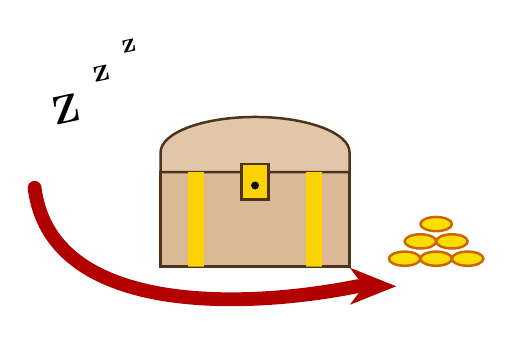
\begin{tikzpicture}[line width=0.9pt]
    % 龙尾巴，绕在宝箱前面
    \draw[red!70!black, line width=5pt, line cap=round]
      (-1.6,1.0) .. controls (-1.4,-0.6) and (1.0,-0.55) .. (2.5,-0.25);
    \filldraw[fill=red!70!black, draw=red!70!black]
      (2.45,-0.05) -- (2.95,-0.25) -- (2.45,-0.45) -- (2.6,-0.25) -- cycle;
    % 宝箱
    \filldraw[fill=brown!55, draw=brown!40!black] (0,0) rectangle (2.4,1.2);
    \filldraw[fill=brown!45, draw=brown!40!black]
      (0,1.2) -- (0,1.45) arc[start angle=180, end angle=0, x radius=1.2, y radius=0.45]
      -- (2.4,1.2) -- cycle;
    \fill[yellow!70!orange] (0.35,0) rectangle (0.55,1.2) (1.85,0) rectangle (2.05,1.2);
    \filldraw[fill=yellow!70!orange, draw=brown!40!black] (1.03,0.85) rectangle (1.37,1.3);
    \fill[black] (1.2,1.03) circle (0.05);
    % 金币
    \foreach \x/\y in {3.1/0.1, 3.5/0.1, 3.9/0.1, 3.3/0.32, 3.7/0.32, 3.5/0.54} {
      \filldraw[fill=yellow!80!orange, draw=orange!80!black]
        (\x,\y) ellipse[x radius=0.2, y radius=0.09];
    }
    % 呼噜声
    \node[font=\Large\bfseries, rotate=12]  at (-1.2,2.0) {Z};
    \node[font=\large\bfseries, rotate=12]  at (-0.75,2.45) {z};
    \node[font=\normalsize\bfseries, rotate=12] at (-0.4,2.8) {z};
  \end{tikzpicture}

  \smallskip
  （嘘——龙在打呼噜）
\end{center}

\subsection{游戏规则}

传说山里的龙洞中藏着一箱金币。你举着火把，站在了洞口。洞里有四个地方（图~\ref{fig:cave-map}）：洞口、岔路口、一个小房间，还有龙穴。宝箱就在龙穴里，一条大红龙正趴在上面睡觉。

\begin{figure}[htbp]
  \centering
  \begin{tikzpicture}[
      place/.style={draw, rounded corners, fill=brown!10, minimum width=22mm,
                    minimum height=12mm, align=center},
      way/.style={thick, {Stealth}-{Stealth}},
    ]
    \node[place]                     (door)  {洞口\\\texttt{\small room = 1}};
    \node[place, right=18mm of door] (fork)  {岔路口\\\texttt{\small room = 2}};
    \node[place, above right=4mm and 18mm of fork] (small) {小房间\\\texttt{\small room = 3}};
    \node[place, below right=4mm and 18mm of fork, fill=red!10] (lair) {龙穴\\\texttt{\small room = 4}};
    \draw[way] (door) -- (fork);
    \draw[way] (fork) -- node[above left, font=\small] {左} (small);
    \draw[way] (fork) -- node[below left, font=\small] {右} (lair);
    \node[right=2mm of small, font=\small, align=left] {墙上挂着\\一把钥匙};
    \node[right=2mm of lair, font=\small, align=left] {龙和宝箱};
  \end{tikzpicture}
  \caption{龙洞地图}
  \label{fig:cave-map}
\end{figure}

每一步，游戏会告诉你在哪里、可以做什么，你输入选项的编号。要小心：火把只够烧 12 步，烧完了就什么也看不见了。至于怎样才能拿到宝箱……自己去试试吧。小提示：龙好像喜欢数学好的人。

\needspace{12\baselineskip}
\subsection{程序}

\codefile{code/ch02/dragon.c}{龙洞寻宝}{lst:dragon}

\subsection{玩一局}

\inputminted[linenos=false]{text}{code/ch02/out/dragon.txt}

（剧透：这只是其中一种玩法。小房间里的钥匙有什么用？你自己去发现吧。）

\subsection{游戏是怎样做出来的}

这个程序有一百多行，看起来很长，其实用到的全是本章讲过的东西。

\paragraph{用变量记住游戏的状态。}程序开头的几个变量，记录了游戏此刻的全部情况：\texttt{room} 记住你在哪里，用 1、2、3、4 代表四个地方；\texttt{has\_key} 记住你有没有钥匙，0 表示没有，1 表示有；\texttt{torch} 记住火把还能烧几步；\texttt{playing} 记住游戏是否还在进行。游戏世界里发生的一切，归根到底就是这几个盒子里的数在变化。

\paragraph{用一个大循环让游戏一直进行下去。}\texttt{while (playing)} 是整个游戏的主循环。只要 \texttt{playing} 不是 0，就一圈一圈地转下去。每一圈都做三件事：
\begin{enumerate}
  \item \textbf{描述}：根据 \texttt{room} 的值，用 \texttt{if}/\texttt{else if} 打印出这个地方的样子和可以做的事；
  \item \textbf{读入}：用 \texttt{scanf} 读入玩家的选择，同时火把少烧一步；
  \item \textbf{更新}：根据“在哪里”和“选了什么”，改变变量的值——走到别的地方就改 \texttt{room}，拿到钥匙就把 \texttt{has\_key} 设为 1，游戏结束就把 \texttt{playing} 设为 0。
\end{enumerate}
玩家看到的“走进山洞”“拿起钥匙”，在程序里不过是 \texttt{room = 2;} 和 \texttt{has\_key = 1;} 而已。

\paragraph{龙的谜题。}龙问的正是 \texttt{for} 循环那一节算过的题。这里用一个 \texttt{for} 循环给玩家 3 次机会，答对了就用 \texttt{break} 提前离开循环，同时把 \texttt{won} 设为 1。循环结束后，如果 \texttt{won} 还是 0，说明 3 次都没答对。

这种“描述—读入—更新”的循环，叫做\emph{游戏循环}。从最简单的文字游戏，到画面精美的大型游戏，用的都是这个结构，只不过大型游戏每秒要转几十圈。还记得第~\ref{chap:hello}~章最后讲到的 CPU 吗？它也在转着一个永不停歇的循环：取指、译码、执行、写回。看来，循环真是计算机世界的心跳。

\subsection{动手改一改}

游戏是你的了，随便改：
\begin{itemize}
  \item 把火把改成只能烧 8 步，看看还能不能拿到宝箱；
  \item 换一道谜题，比如“1 加到 1000 等于几”，或者让龙问你的生日；
  \item 增加一个地方，比如小房间后面的地下河。给它一个新的 \texttt{room} 编号，在“描述”和“更新”两部分各加一段 \texttt{else if}；
  \item 增加一个新的物品，比如一把剑。用一个新的变量 \texttt{has\_sword} 记住有没有拿到它。
\end{itemize}
改完了，运行 \texttt{make test} 看看原来的玩法还对不对。如果你改了游戏的规则，测试报告“失败”是正常的，那说明它在认真检查。

\section{小结}

\begin{itemize}
  \item 变量是贴了标签的盒子。\texttt{int} 型的变量装整数；\texttt{=} 是赋值，把右边的值放进左边的变量。
  \item 算术运算有 \texttt{+ - * / \%}。整数相除只要商，\texttt{\%} 取余数。
  \item \texttt{printf} 用 \texttt{\%d} 打印整数，\texttt{scanf} 用 \texttt{\%d} 读入整数，变量名前要加 \texttt{\&}。
  \item \texttt{if}/\texttt{else if}/\texttt{else} 根据条件选择要执行的代码。判断相等用 \texttt{==}，不是 \texttt{=}；编译时加上 \texttt{-Wall}。
  \item \texttt{\&\&}、\texttt{||}、\texttt{!} 组合条件。C 语言中 0 表示不成立，非 0 表示成立。
  \item \texttt{while} 在条件成立时重复执行；\texttt{for} 适合“从几数到几”；\texttt{break} 提前离开循环。死循环用 \texttt{Ctrl+C} 停止。
  \item 一个游戏，就是用变量记住状态，在一个循环中不断地描述、读入、更新。
\end{itemize}

\section*{练习}

\begin{enumerate}
  \item 写一个程序，读入一个秒数，比如 3725，打印出它是几小时几分几秒（1 小时 2 分 5 秒）。提示：用 \texttt{/} 和 \texttt{\%}。
  \item 修改代码~\ref{lst:sum}，算出 1 到 100 中所有偶数的和。（答案是 2550。）
  \item 用 \texttt{for} 循环打印九九乘法表。
  \item 修改代码~\ref{lst:guess}，如果猜了 7 次还没猜中，就告诉玩家答案并结束游戏。
  \item 修改代码~\ref{lst:triangle}，打印一个倒过来的三角形。
  \item 给龙洞寻宝增加一个新的地方和一件新的物品，再写一段测试，加进 \texttt{test.sh}。
\end{enumerate}
